\documentclass[10pt,a4paper]{article}
\usepackage{caratula}
\usepackage{geometry}
\renewcommand\familydefault{\sfdefault} % Default family: serif 
\usepackage[usenames,dvipsnames]{xcolor}
\usepackage{tikz}
\usepackage{soul}
\usetikzlibrary{calc} 
\usetikzlibrary{arrows, decorations.markings,positioning,backgrounds,shapes}
\definecolor{EMP}{HTML}{77DD77} % Green1
\definecolor{NOR}{HTML}{06500C} % Green2
\usepackage{ulem}
\renewcommand{\ULdepth}{3pt}
\usepackage{tikz-dependency}
\usepackage{graphicx} 
\usepackage{indentfirst}
\setlength{\parindent}{12pt}

%\usetikzlibrary{positioning}




\titulo{TP1 }
\subtitulo{Relación PBI - Cantidad de sedes Argentinas en el exterior}

\fecha{\today}

\materia{Laboratorio de Datos}
\grupo{GRUPO 100}

\integrante{Chapana Puma, Joselin Miriam}{1197/21}{yoselin.chapana@gmail.com}
\integrante{Martinelli, Lorenzo}{364/23}{martinelli.lorenzo12@gmail.com}
\integrante{Padilla, Ramiro Martin}{1636/21}{ramiromdq123@gmail.com}

\graphicspath{{../static/}}


\begin{document}
\newgeometry{margin=2cm}

\maketitle

\restoregeometry
%\newgeometry{top=3cm,bottom=3cm,right=3cm,left=3cm} para editar margenes menos del titulo 


\section{Resumen}
este es el resumen


\section{Introducción} \vspace{0.1cm}

\subsection{Objetivo y Fuente} \vspace{0.1cm}

El objetivo principal de este trabajo es encontrar una relación entre la cantidad de sedes de Argentina en un país y su PBI, para esto, trabajaremos con los siguientes datos, 

\begin{itemize}
	\item PBI per cápita de los paises (1)
	\item Representaciones Argentinas en el exterior, donde tenemos, Datos básicos de las sedes, Datos completos de sedes y secciones (2)
\end{itemize}

\noindent (1) https://data.worldbank.org/indicator/NY.GDP.PCAP.CD \vspace {0.1cm}

\noindent (2) https://datos.gob.ar/dataset/exterior-representaciones-argentinas \vspace{0.1cm}
 
\subsection{Procedimiento}

\indent Este trabajo tendrá varias etapas, comenzando con el planteo de un Diagrama de Entidad Relacional (DER) adecuado al objetivo de nuestro trabajo, continuando con la elaboración y normalización de un Modelo Relacional. Además, de llevar a cabo una limpieza de los datos utlizando ciertas metricas, en particular, utilizaremos el método GQM. \par

Una vez tengamos los datos limpios y el modelo normalizado, pasaremos al procesamiento y visualización de datos en Python utilizando librerias como Pandas, Inlinesql, Matplotlib entre otras con el fin de elaborar nuestras conclusiones, ¿Será mayor el PBI de aquellos paises con sedes Argentinas? ¿Influirá la cantidad de sedes y/o secciones de estas?.  

\newpage

\section{Procesamiento de Datos} \vspace{0.2cm}

\subsection{Diagrama de Entidad Relacional} \vspace{0.2cm}

Una vez planteado nuestro objetivo, nos encargamos de ver que datos necesitabamos para alcanzarlo, y como estarian representados. Para esto, elaboramos el siguien diagrama de entidad
relacional.  \vspace{0.2cm}

\begin{figure}[ht]
	\centering
	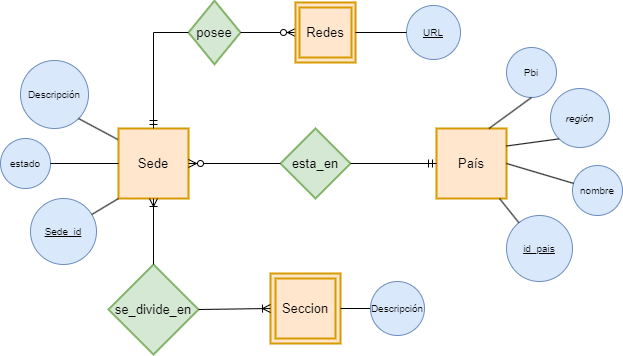
\includegraphics[width=1\textwidth]{DERPBI.png}
	\caption{Diagrama de Entidad Relacional}
	\label{fig:ejemplo}
\end{figure}

Como se puede ver en la Figure 1, consideramos que,

\begin{itemize}
	\item Una sede esta en un país y solo en uno.
	\item Un País puede tener muchas o ninguna sede.
	\item Las secciones existen pues existen las sedes, entonces, lo consideramos una entidad debil.
	\item Una sección puede estar en una o muchas Sedes, por ejemplo, la Embajada en Brasil y en Chile tiene su sección Administración.
	\item Una sede tiene al menos una sección.
	\item Cuando hablamos de Redes, hablamos mas de un perfil en una red social, por lo tanto, una red puede pertenecer a una y solo una sede.
\end{itemize}


\newpage

\subsection{Modelo Relacional} \vspace{0.2cm}

Una vez que tenemos nuestro esquema gráfico, pasamos al planteo del modelo relacional. Notar que, las flechas representan las Foreign Keys y aquellos atributos 
subrayados representan las Primary Keys. En todas las relaciones, exceptuando a País, las Claves coinciden con las claves candidatas, esto se debe a que en País consideramos también a 
nombrePais como una posible clave. \par
Otro detalle a tomar en cuenta, es que decidimos separar la relación País(IdPais, región, nombre, Pbi) puesto que perdiamos la 2FN a raíz de que 
al ser nombre una clave candidata, región y Pbi dependian parcialmente de la clave primaria. \vspace{0.4cm}

\newbox\ubox

\begin{tikzpicture}[
    EMP/.style={% Style for empatized boxes
        rectangle, line width =1pt,
        anchor=west,
        underline, % new property
        align=center,
        text=Black,
        minimum height=.8cm,
        text height=1.7ex,
            text depth=.25ex,
        fill=EMP,
        draw=black,
        },
    NOR/.style={% Style for normal boxes.
        rectangle, 
        line width =1pt,
        anchor=west,
        align=left,
        minimum height=.6cm,
        text height=1.5ex,
            text depth=.25ex,
            text=white,
        fill=NOR,
        draw=black,
        inner ysep=5pt
        },
    underline/.append style={% define new style property
        execute at begin node={%
            \setbox\ubox=\hbox\bgroup
            },
            execute at end node={%
                \egroup\uline{\box\ubox}%
                }
             },
    ] % Uff that is all the configuration for tickzpicture xD

% Define an brute force objet "Frame"
% Variables 1:Position, 2: Identifier, 3: Title of frame 4: Subframe/Boxtype
 \def\Frame(#1)#2[#3]#4{%
  \begin{scope}[shift={(#1)}] 
      \node[font=\bf, anchor=west] (Title) at (-0.2,0.7) {#3}; 
       \edef\k{0}% Variable for box positión
       \edef\x{0}% Variable for named coordinate centering - below box
       \foreach \id/\style in {#4} {%enter sub frame data Name/Boxtype ,Name2/Boxtype | An space before Boxtype is needed 
            \node[\style] (h) at (\k pt,0) {\id}; %  % Draw a node depending on the variables.
            \pgfmathparse{\k+0.5*width{"\id"}+3.4pt} % Uses the textwidth to calculate named coordinate  
            \xdef\x{\pgfmathresult} % The resul is saved in the variable \x
            \draw (\x pt,-0.4) coordinate (\id#2); %Create a named coordinate concatenated: "sub frame data Name"+"identifier"
            \pgfmathparse{\k+width{"\id"}+6.8pt}% Calculate positión for each subframe box.       
        \xdef\k{\pgfmathresult}% Save the value to be added to the next iteration value.
       }    
  \end{scope}
}% disadvantages: Is not posible to use Frame data Name like: Name_another_desc instead I use Name-another-desc

% Start drawing
% \node[EMP node] (dm) at (0,0) {{Sometext/EMP,another/EMP}};
  \Frame(0,0){3}[PAIS]{
    IdPais/EMP,
    NombrePais/NOR};

 \Frame(0,-2.5){1}[SEDE]{%first frame identified as 1 named EMPLOYEE
    IdSede/EMP,% see that it is necessary to add a space
    IdPais/NOR,
    Descripción/NOR,
    Estado/NOR}; 

 \Frame(0,-5){2}[REDES]{
    IdSede/EMP,
    Urls/EMP};  

 \Frame(0,-7.5){4}[REGION]{
    IdPais/EMP,
    Region/NOR};

  \Frame(0,-10){5}[SECCIONES]{
    IdSede/EMP,
    SeccionDescripcion/EMP};     

 \Frame(0,-12.5){6}[PBI]{
    IdPais/EMP,
    PBI-2022/NOR,}; 

% Start drawing arrows:
% In this part I use the named coordinates to draw the arrows.
    \draw[thick,<-,thick,>=latex] % From Essn6 to Ssn1  
        (IdSede1)++(0.1,0) -- ++(0,-.55) -- ++(4.5,0) coordinate (inter) %inter is the name of coordinate register
        -- (IdSede2 -| inter) -- ++(0,-0.4) coordinate (inter)  % to calculate intersections.
        -- (IdSede2 |- inter) --++(0,0.4); %
        
    \draw[thick,<-,thick,>=latex]
        (IdPais3) -- ++(0,-.675) -- ++(5.2,0) coordinate (inter) 
        -- (IdPais4 -| inter) -- ++(0,-0.2) coordinate (inter) 
        -- (IdPais4 |- inter) --++(0,0.2); %

     \draw[thick,<-,thick,>=latex]
        (IdSede1)++(-0.3,0) -- ++(0,-.85) -- ++(4.3,0) coordinate (inter) 
        -- (IdSede5 -| inter) -- ++(0,-0.2) coordinate (inter) 
        -- (IdSede5|- inter) --++(0,0.2); %.
        
     \draw[thick,<-,thick,>=latex]
        (IdSede1)++(-0.3,0) -- ++(0,-.85) -- ++(4.3,0) coordinate (inter) 
        -- (IdSede5 -| inter) -- ++(0,-0.2) coordinate (inter) 
        -- (IdSede5|- inter) --++(0,0.2); %.

    \draw[thick,<-,thick,>=latex] % From Essn6 to Ssn1  
        (IdPais3)++(0.2,0) -- ++(0,-.5) -- ++(5.2,0) coordinate (inter) %inter is the name of coordinate register
        -- (IdPais1 -| inter) -- ++(0,-0.4) coordinate (inter)  % to calculate intersections.
        -- (IdPais1 |- inter) --++(0,0.45); %

    \draw[thick,<-,thick,>=latex] % From Essn6 to Ssn1  
        (IdPais3)++(-0.2,0) -- ++(0,-.85) -- ++(5.8,0) coordinate (inter) %inter is the name of coordinate register
        -- (IdPais6 -| inter) -- ++(0,-0.4) coordinate (inter)  % to calculate intersections.
        -- (IdPais6 |- inter) --++(0,0.45); %

        
\end{tikzpicture} \vspace{0.2cm}

\newpage

\subsection{Normalización} \vspace{0.1cm}

Con los datos aún sin limpiar, nuestro modelo no está en 1FN, pues tiene columnas con varios datos en cada celda, por ejemplo, 
todas las redes sociales de una sede aparecen en una misma celda separadas por "//". Sin embargo, podemos mostrar nuestro modelo respeta la 2FN Y 3FN. 
Para esto, veamos sus dependecias funcionales. \vspace{0.2cm}

\depstyle{lvl}{%
    edge height=2.5ex,
    % edge unit distance=#1*2.5ex, % Another way of controlling the appearance of the edges.
    edge below,
    edge horizontal padding=0,
    edge vertical padding=(#1-1)*3ex,
    text only label, % No need for label for functional dependencies.
    edge slant=0, % Right angles
    rounded corners=0,
    edge style={>=triangle 60} % Change the style of the arrowheads.
}
\tikzset{
    matrix/.append style={column sep=0.4cm} % Adding some distance between the attributes.
}
\tikzstyle{TxtBook}=[% Style to mimic the textbook Fundamentals of Database Systems.
    column sep=0cm, % No distance between two attributes.
    nodes={%
        fill=gray!20,
        draw=black,
        thick,
        inner xsep=3ex,
        inner ysep=1ex
    }
]
\tikzstyle{TxtBookChico}=[% Style to mimic the textbook Fundamentals of Database Systems.
    column sep=0cm, % No distance between two attributes.
    nodes={%
        fill=gray!20,
        draw=black,
        thick,
        inner xsep=1.2ex,
        inner ysep=1ex
    }
]


\textbf{Sede} \vspace{0.1cm}

\begin{dependency}
    \raggedright
    \begin{deptext}[TxtBookChico] % Applying the TxtBook style.
        \textbf{\underline{idSede}}  \& idPaís \& Descripción \& Estado \\
    \end{deptext}
    \depedge[lvl=1]{1}{2}{}
    \depedge[lvl=1]{1}{3}{}
    \depedge[lvl=1]{1}{4}{}
\end{dependency} \vspace{0.3cm}

Veamos que la unica dependencia funcional que tenemos es, \vspace{0.3cm}

 idSede $\rightarrow$ $\{$idPaís, Descipción, Estado$\}$ \vspace{0.3cm}

Puesto que con el id de un País no podemos inferir la descripción de una sede en particular ni su estado. Tampoco podemos inferir los demas atributos
a partir de la descripción de una sede pues consideramos que podria haber descripciones repetidas o faltantes y no son suficiente para identificarlas. 
Por lo tanto, tenemos que todos los atributos no primos dependen de la Clave Primaria y está en 2FN, mas aún, está en 3FN. Notar además, que la DF es minimal puesto
que posee un solo atributo en su lado izquierdo. \vspace{0.3cm}

El detalle comentando en el modelo relacional en cuanto a la estructura y el porque de nuestra elección se puede ver en la siguiente tabla. \vspace{0.3cm}

\textbf{País} 
 \vspace{0.1cm}

\begin{dependency}
    \raggedright
    \begin{deptext}[TxtBook] % Applying the TxtBook style.
        \textbf{\underline{idPaís}}  \& NombrePaís \& Región \& PBI  \\
    \end{deptext}
    \depedge[lvl=1]{1}{2}{}
    \depedge[lvl=1]{1}{3}{}
    \depedge[lvl=1]{1}{4}{}
    \depedge[lvl=2]{2}{3}{}
    \depedge[lvl=2]{2}{4}{}
\end{dependency} \vspace{0.3cm}

Es fácil notar que con la DF mas externa, estamos perdiendo la 2FN y por ende la 3FN, puesto que tenemos atributos no primos que dependen parcialmente de la clave primaria.
Por lo tanto, nuestra solución fue dividir en tablas como se muestra a continuación, \vspace{0.3cm}


\textbf{País} 
\vspace{0.1cm}

\begin{dependency}
    \raggedright
    \begin{deptext}[TxtBook] % Applying the TxtBook style.
        \textbf{\underline{idPaís}}  \& NombrePaís\\
    \end{deptext}
    \depedge[lvl=1]{1}{2}{}
\end{dependency} \vspace{0.3cm}

\textbf{Región} 
\vspace{0.1cm}

\begin{dependency}
    \raggedright
    \begin{deptext}[TxtBook] % Applying the TxtBook style.
        \textbf{\underline{idPaís}} \& Región  \\
    \end{deptext}
    \depedge[lvl=1]{1}{2}{}
\end{dependency} \vspace{0.3cm}


\textbf{PBI} 
\vspace{0.1cm}

\begin{dependency}
    \raggedright
    \begin{deptext}[TxtBook] % Applying the TxtBook style.
        \textbf{\underline{idPaís}} \& PBI  \\
    \end{deptext}
    \depedge[lvl=1]{1}{2}{}
\end{dependency} 

De esta manera, estamos respetando la 2FN puesto que dependemos completamente de la PK y, en 3FN pues idPais es SK en todas las relaciones . Además, las DF detalladas son minimales puesto que dependen de un solo atributo.

\vspace{3mm}
\textbf{Sección} 

\begin{dependency}
    \raggedright
    \begin{deptext}[TxtBook] % Applying the TxtBook style.
        \textbf{\underline{IdSede}}  \& \textbf{\underline{Sección}}  \\
    \end{deptext}
\end{dependency}

\vspace{3mm}
\textbf{Redes} 

\begin{dependency}
    \raggedright
    \begin{deptext}[TxtBook] % Applying the TxtBook style.
        \textbf{\underline{IdSede}}  \& \textbf{\underline{redURL}}  \\
    \end{deptext}
	\depedge[lvl=1]{2}{1}{}
\end{dependency} \vspace{0.3cm}

Notemos que en Sección relaciones no podemos establecer dependendencias funcionales puesto que solo con el IdSede yo no puedo inferir una sección, y tampoco
puedo realizar el camino inverso. Por otro lado, en Redes si puedo determinar la sede a partir de su url sin embargo, no puedo hacer el camino inverso pues tengo más de
una url asociada a una unica sede.  \par
Una vez hecha la aclaración, podemos ver que Sección esta en 3FN pues no posee DF. Y, por otro lado, Redes está también en 3FN pues IdSede es un atributo primo.

\section{Decisiones tomadas}


\section{Análisis de datos}


\section{Conclusiones}

\end{document}